\documentclass[tikz, border=10pt]{standalone}
\usepackage{tikz}
\usetikzlibrary{shapes.geometric, arrows.meta, positioning, fit, backgrounds}

\definecolor{mhacolor}{RGB}{34, 150, 100}
\definecolor{mlpcolor}{RGB}{190, 80, 50}
\definecolor{normcolor}{RGB}{120, 90, 170}
\definecolor{addcolor}{RGB}{80, 80, 80}
\definecolor{arrowcolor}{RGB}{60, 60, 60}
\definecolor{bgblock}{RGB}{245, 255, 248}

\tikzset{
  block/.style={rectangle, rounded corners=4pt, minimum width=3.2cm, minimum height=0.75cm, text centered, font=\small\bfseries, draw, thick},
  normblock/.style={block, fill=normcolor!20, draw=normcolor!70, text=normcolor!80!black},
  mhablock/.style={block, fill=mhacolor!20, draw=mhacolor!70, text=mhacolor!80!black},
  mlpblock/.style={block, fill=mlpcolor!20, draw=mlpcolor!70, text=mlpcolor!80!black},
  addblock/.style={circle, minimum size=0.55cm, text centered, font=\small\bfseries, fill=addcolor!15, draw=addcolor!60, text=addcolor},
  ioblock/.style={rectangle, rounded corners=2pt, minimum width=3.2cm, minimum height=0.6cm, text centered, font=\small, fill=gray!15, draw=gray!50},
  arr/.style={-{Stealth[length=5pt]}, thick, color=arrowcolor},
  skiparr/.style={-{Stealth[length=5pt]}, thick, color=addcolor!70, dashed}
}

\begin{document}
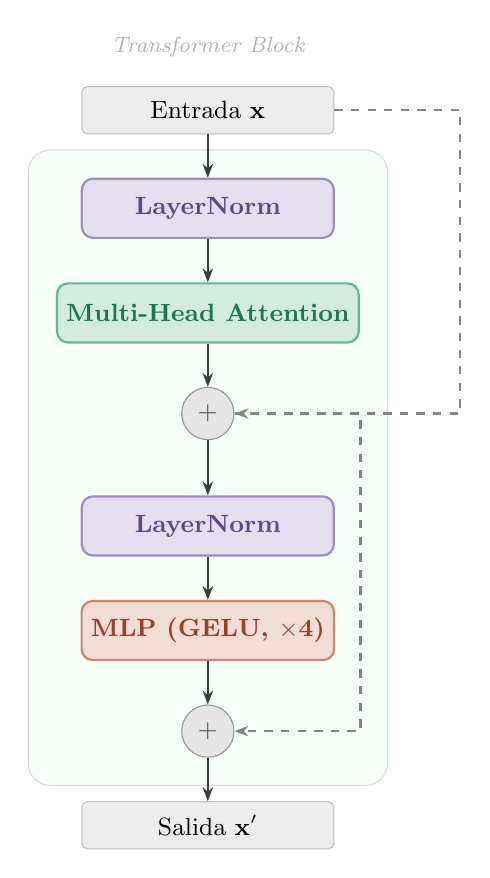
\begin{tikzpicture}[node distance=0.55cm]

  \node[font=\footnotesize\itshape, text=gray!60] (title) {Transformer Block};
  \node[ioblock, below=0.25cm of title] (input) {Entrada $\mathbf{x}$};

  \node[normblock, below=of input]      (ln1)  {LayerNorm};
  \node[mhablock,  below=of ln1]        (mha)  {Multi-Head Attention};
  \node[addblock,  below=of mha]        (add1) {$+$};

  \node[normblock, below=0.7cm of add1] (ln2)  {LayerNorm};
  \node[mlpblock,  below=of ln2]        (mlp)  {MLP (GELU, $\times$4)};
  \node[addblock,  below=of mlp]        (add2) {$+$};

  \node[ioblock, below=of add2]         (output) {Salida $\mathbf{x}'$};

  \draw[arr] (input) -- (ln1);
  \draw[arr] (ln1)   -- (mha);
  \draw[arr] (mha)   -- (add1);
  \draw[arr] (add1)  -- (ln2);
  \draw[arr] (ln2)   -- (mlp);
  \draw[arr] (mlp)   -- (add2);
  \draw[arr] (add2)  -- (output);

  \draw[skiparr] (input.east) -- ++(1.6,0) |- (add1.east);
  \draw[skiparr] (add1.east)  -- ++(1.6,0) |- (add2.east);

  \begin{scope}[on background layer]
    \node[fill=bgblock, draw=gray!30, rounded corners=8pt, inner sep=10pt,
          fit=(ln1)(mha)(add1)(ln2)(mlp)(add2)] (border) {};
  \end{scope}

\end{tikzpicture}
\end{document}
